\section*{سوال ۴}

در یک فروشگاه تحت وب، کسب و کار مربوطه وظیفه واسطه‌گری را بر عهده دارد و تعداد زیادی مشتری را به تعداد زیادی انباردار متصل می‌کند. هم مشتریان و هم انبارداران در این سیستم دارای حساب و کیف پول هستند، و هر خرید به طور مستقیم پول را از کیف پول مشتری به کیف پول فروشنده منتقل می‌کند (بدون هیچ هزینه‌ای).

مدل زیرساختی که برای این فروشگاه تعریف شده است به عنوان مدل backend شناخته می‌شود و برای بخشی از کد زیرسیستم طراحی شده است. برای سهولت در توضیح سوال، بسیاری از جزئیات (داده‌ها و عملیات کلاس‌ها) حذف شده‌اند و تمرکز بر روی کلاس‌ها و روابط بین آن‌ها است.

\begin{figure}[h]
	\centering
	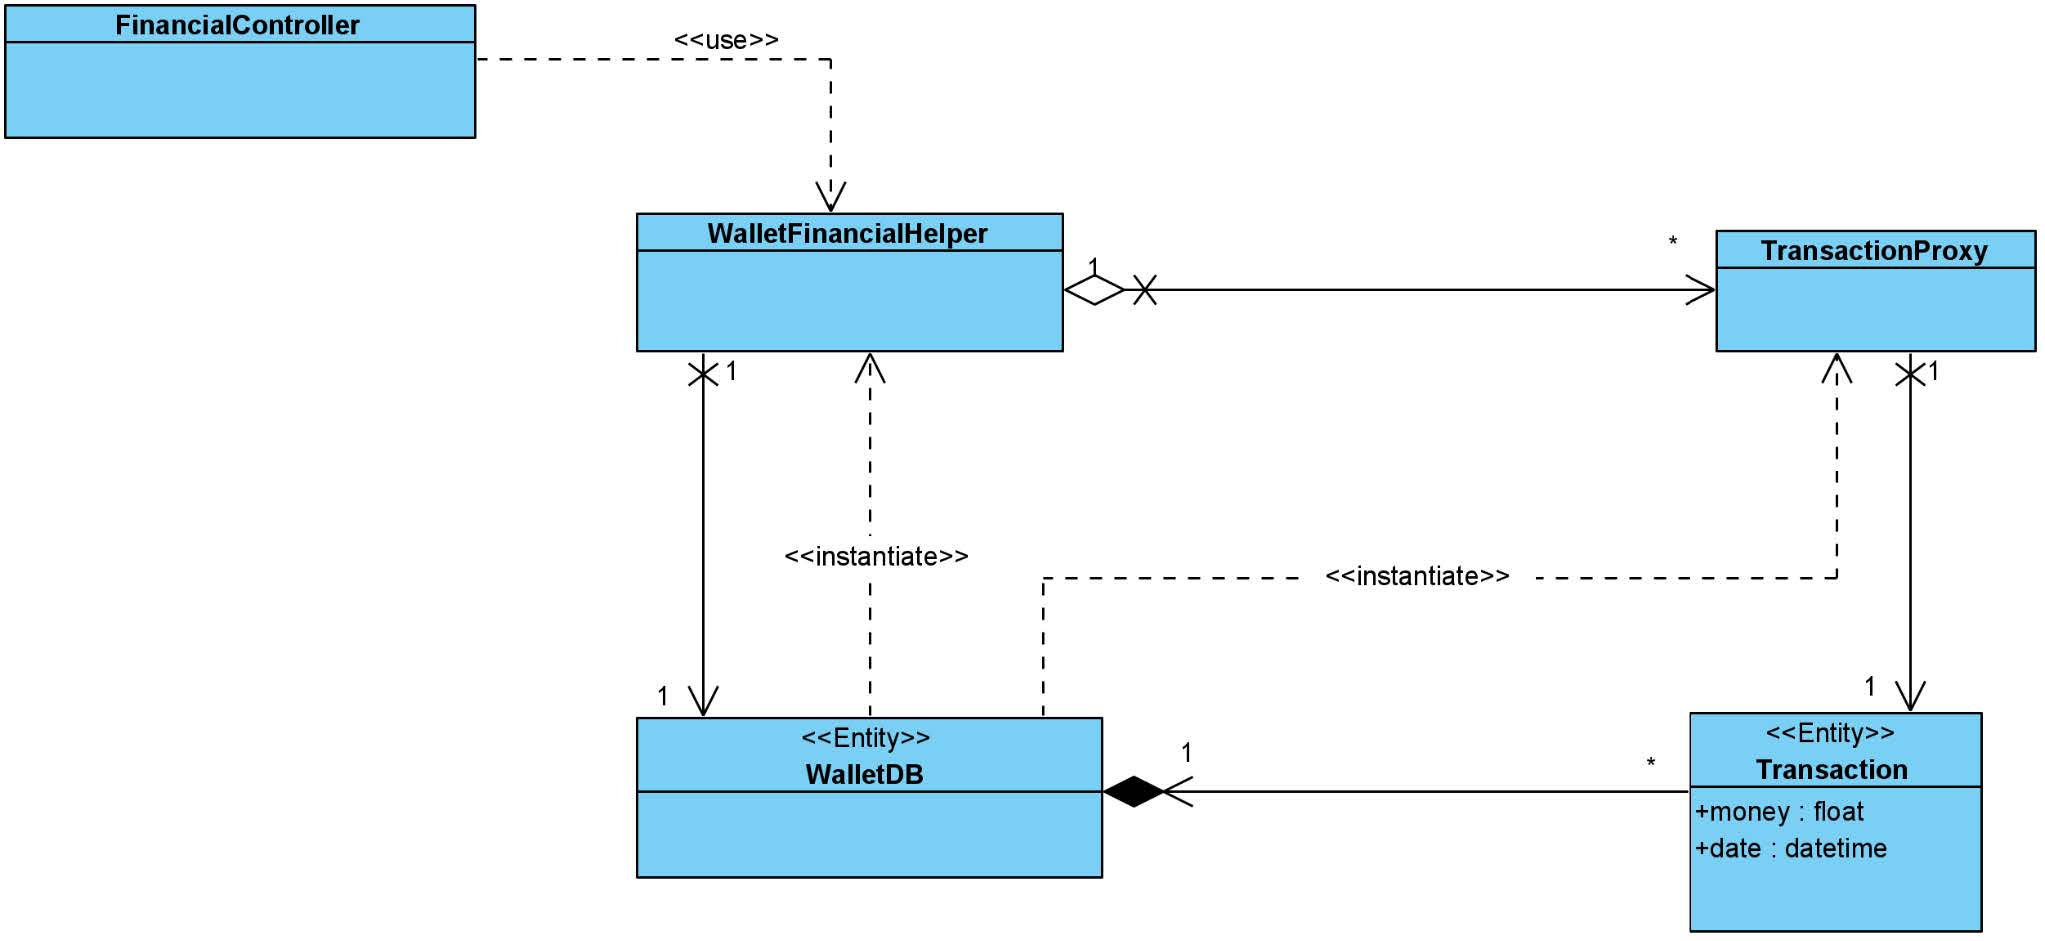
\includegraphics{pic1.jpg}
	\label{fig:label4}
\end{figure}

\subsection*{۱. بازسازی مدل تحلیل}
مدل تحلیل متناظر با مدل طراحی فوق از دست رفته است. آن را بازسازی کنید. (نکته: مدل تعبیه شده باید ساده‌تر و کوچک‌تر از مدل طراحی باشد.)

\subsection*{۲. استفاده از الگوهای تحلیل فاولر}
در فصل‌های ۸ تا ۱۱ کتاب «پرسمن»، به الگوهای تحلیل - به خصوص الگوهای تحلیل فاولر - اشاره شده است. کتاب فاولر را می‌توانید از لینک مذکور دریافت کنید. از الگوی «موجودی و حسابداری - تراکنش» (فصل ۶ کتاب الگوهای تحلیل فاولر) استفاده کنید و مدل تحلیلی را که در بخش ۱ ایجاد کردید، با استفاده از این الگو غنی‌سازی کنید.

\begin{figure}[h]
	\centering
	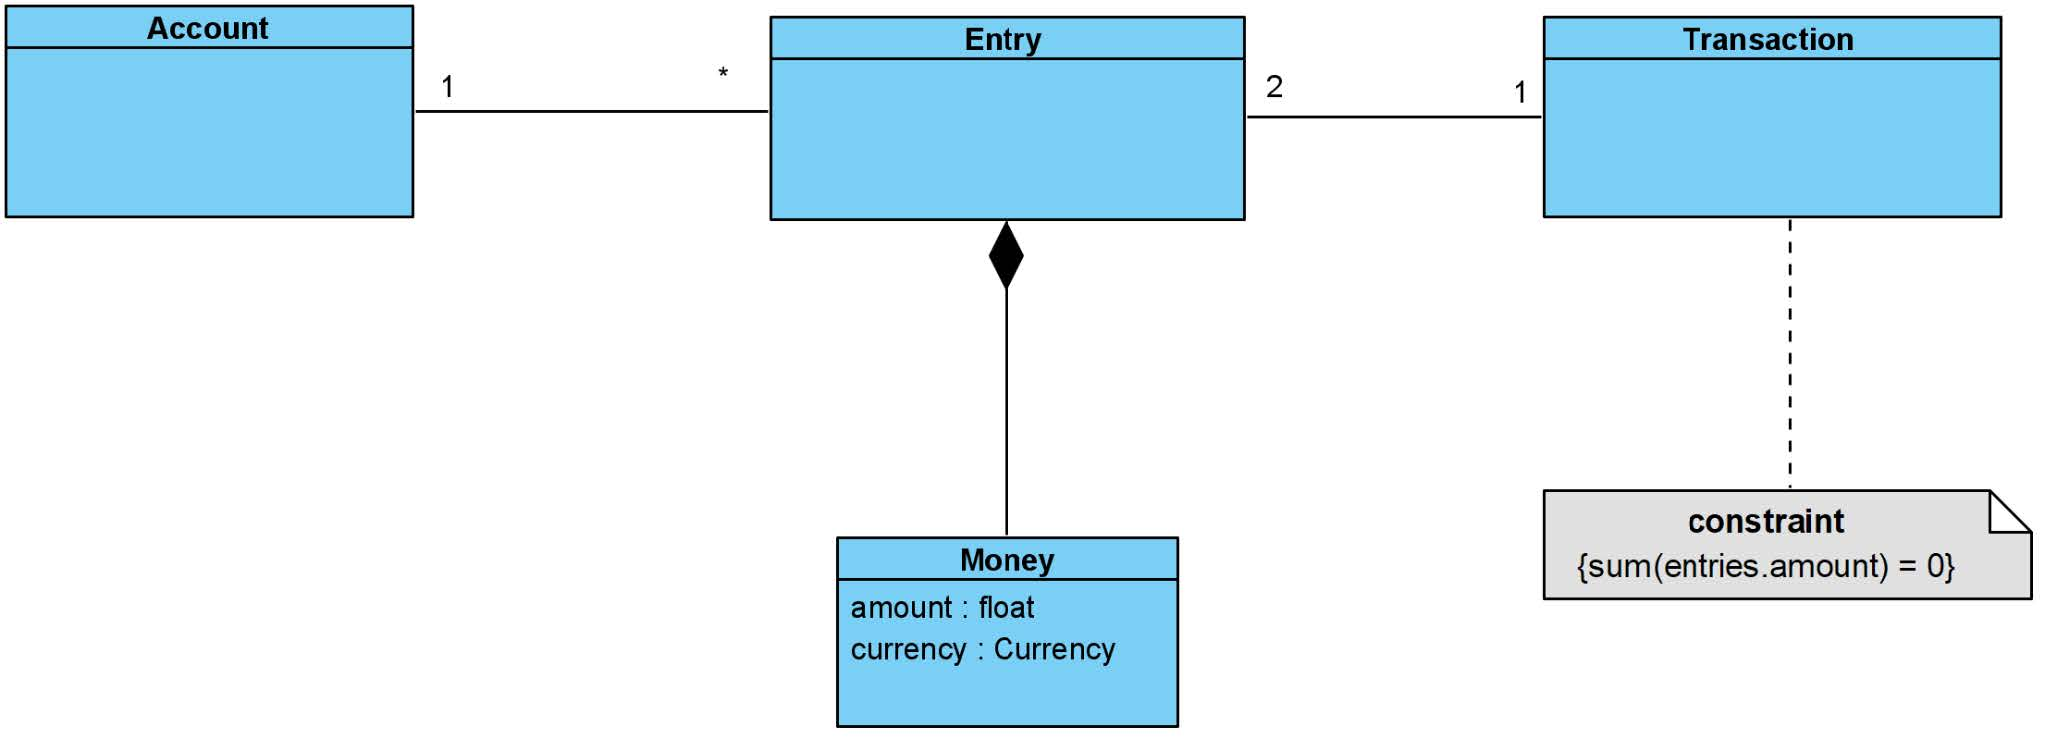
\includegraphics{pic2.jpg}
	\label{fig:label4}
\end{figure}

\subsection*{۳. توجیه بهبود‌ها}
دو مورد از بهبود‌هایی که این الگو به ارمغان می‌آورد را توجیه کنید.

\section*{جواب سوال ۴}

\subsection*{جواب بخش اول}

\begin{figure}[H]
	\centering
	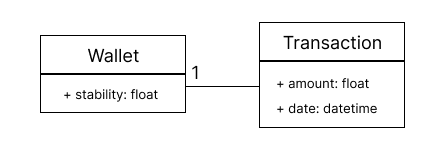
\includegraphics{pic3.png}
	\label{fig:label4}
\end{figure}

\subsection*{جواب بخش دوم}

\begin{figure}[H]
	\centering
	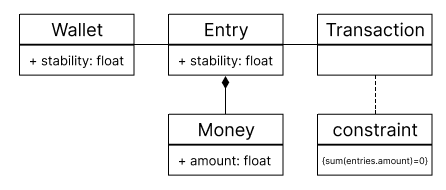
\includegraphics{pic4.png}
	\label{fig:label4}
\end{figure}

\subsection*{جواب بخش سوم}

\subsubsection*{بهبود اطمینان از صحت تراکنش‌ها}
در مدل قبلی، هر تراکنش به صورت جداگانه ایجاد می‌شد، بدون اطمینانی از اینکه عملیات مرتبط با آن قرینه و صحیح باشد. این امر خطر ایجاد تراکنش‌های نامعتبر را افزایش می‌داد، که می‌توانست منجر به خلق یا حذف نادرست مقداری پول شود. با اعمال الگوی فاولر، هر تراکنش به وضوح با یک عملیات متقابل مرتبط می‌شود. این امر به وسیله تعریف دو transaction برای هر entry و تضمین اینکه جمع مبالغ در هر entry صفر باشد، اطمینان از صحت و تعادل مالی را فراهم می‌کند.


\subsubsection*{افزایش شفافیت و ردیابی تراکنش‌ها}

در مدل قبلی، برای هر طرف در تراکنش، یک transaction جداگانه ایجاد می‌شد و رابطه میان این transaction‌ ها مشخص نبود. در نتیجه، دسترسی به اطلاعات کامل تراکنش برای هر دو طرف دشوار بود. با به کارگیری الگوی جدید، هر transaction به یک entry مرتبط است و هر entry شامل تمام transaction‌ های مربوط به یک مبادله مالی است. این ساختار جدید امکان ردیابی و شفافیت بیشتری را در مورد جریان‌های مالی فراهم می‌کند، زیرا تمام مبادلات مالی مرتبط با یک فرد به راحتی قابل شناسایی است.